\documentclass{beamer}
\usepackage[utf8]{inputenc}

\usetheme{Madrid}
\usecolortheme{default}
\usepackage{amsmath,amssymb,amsfonts,amsthm}
\usepackage{txfonts}
\usepackage{tkz-euclide}
\usepackage{listings}
\usepackage{adjustbox}
\usepackage{array}
\usepackage{tabularx}
\usepackage{gvv}
\usepackage{lmodern}
\usepackage{circuitikz}
\usepackage{tikz}
\usepackage{graphicx}

\setbeamertemplate{page number in head/foot}[totalframenumber]

\title{1.8.18}
\date{August 30, 2025}
\author{EE25BTECH11001 - Aarush Dilawri}

\begin{document}

\frame{\titlepage}

\begin{frame}{Question}
\textbf{Question}:\\
Find the values of $y$ for which the distance between the points $\vec{P}(2,-3)$ and $\vec{Q}(10,$y$)$ is 10 units.
\end{frame}

\begin{frame}{Solution}
\textbf{Solution}:\\
We are given the points
\begin{align}
\vec{P} = \myvec{2\\-3}, \quad 
\vec{Q} = \myvec{10\\$y$}
\end{align}
\end{frame}

\begin{frame}{Step 1}
The distance between them is $10$ units, so
\begin{align}
\|\vec{P}-\vec{Q}\| &= 10
\end{align}
\end{frame}

\begin{frame}{Step 2}
Squaring both sides,
\begin{align}
\|\vec{P}-\vec{Q}\|^2 &= \|\vec{P}\|^2 + \|\vec{Q}\|^2 + 2\vec{P}^T\vec{Q} = 10^2
\end{align}
\end{frame}

\begin{frame}{Step 3}
Substituting,
\begin{align}
13 + (10 + y)^2 + 2(20 -3y) = 100\\
\implies y = 3 \quad \text{or} \quad y = -9
\end{align}
\end{frame}

\begin{frame}{Figure}
See Fig. 0 ,
\begin{figure}[H]
\begin{center}
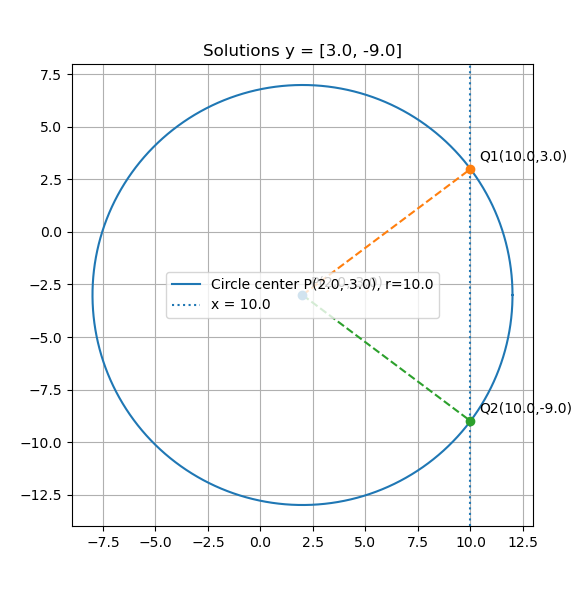
\includegraphics[width=0.6\columnwidth]{figs/fig.png}
\end{center}
\caption{}
\label{fig:Fig1}
\end{figure}
\end{frame}



\begin{frame}[fragile]{C Code (code.c)}
\begin{lstlisting}[language=C]
#include<math.h>

int find_y(double x1, double y1, double x2, double d, double *y_out1, double *y_out2) {
    double dx = x1 - x2;
    double inside = d * d - dx * dx; /* (y1 - y)^2 = inside */

    if (inside < 0.0) {
        /* No real solutions */
        return 0;
    } else if (inside == 0.0) {
        /* exactly one solution (double root) */
        *y_out1 = y1;
        *y_out2 = y1;
        return 1;
\end{lstlisting}
\end{frame}
\begin{frame}[fragile]{C Code (code.c)}
\begin{lstlisting}[language=C]
    } else {
        double r = sqrt(inside);
        *y_out1 = y1 + r;
        *y_out2 = y1 - r;
        return 2;
    }
}
\end{lstlisting}
\end{frame}

\begin{frame}[fragile]{Python Code (code.py)}
\begin{lstlisting}[language=Python]
import numpy as np
import matplotlib.pyplot as plt

# Given values
x1, y1 = 2, -3
x2 = 10
d = 10

# Solve for y values
dx = x1 - x2
inside = d**2 - dx**2
if inside < 0:
    y_solutions = []
else:
    r = np.sqrt(inside)
    y_solutions = [y1 + r, y1 - r]
\end{lstlisting}
\end{frame}
\begin{frame}[fragile]{Python Code (code.py)}
\begin{lstlisting}[language=Python]
print("Solutions for y:", y_solutions)

# Circle centered at P with radius d
theta = np.linspace(0, 2*np.pi, 400)
circ_x = x1 + d * np.cos(theta)
circ_y = y1 + d * np.sin(theta)

# Plot
plt.figure(figsize=(6,6))
plt.plot(circ_x, circ_y, label=f'Circle: center P({x1},{y1}), r={d}')
plt.axvline(x=x2, linestyle=':', color='gray', label=f'x = {x2}')

# Point P
plt.scatter([x1], [y1], color='red', zorder=5)
plt.annotate(f'P({x1},{y1})', (x1,y1), textcoords="offset points", xytext=(6,6))
\end{lstlisting}
\end{frame}
\begin{frame}[fragile]{Python Code (code.py)}
\begin{lstlisting}[language=Python]
for i, yq in enumerate(y_solutions):
    plt.scatter([x2], [yq], color='blue', zorder=6)
    plt.annotate(f'Q{i+1}({x2},{yq:.1f})', (x2,yq), textcoords="offset points", xytext=(6,6))
    plt.plot([x1, x2], [y1, yq], linestyle='--', color='green')

plt.gca().set_aspect('equal', 'box')
plt.grid(True)
plt.legend()
plt.title('Specific Case: P(2,-3), Q(10,y), Distance=10')
plt.show()

\end{lstlisting}
\end{frame}
\begin{frame}[fragile]{Python Code (nativecode.py)}
\begin{lstlisting}[language=Python]
import ctypes
from ctypes import c_double, POINTER, byref, c_int
import numpy as np
import matplotlib.pyplot as plt
from pathlib import Path
import sys

lib_path = Path(__file__).with_name('libfindy.so')
lib = ctypes.CDLL(str(lib_path))

lib.find_y.argtypes = [c_double, c_double, c_double, c_double, POINTER(c_double), POINTER(c_double)]
lib.find_y.restype = c_int
\end{lstlisting}
\end{frame}
\begin{frame}[fragile]{Python Code (nativecode.py)}
\begin{lstlisting}[language=Python]
def find_y_py(x1, y1, x2, d):
    """Wrapper around the C function. Returns a list of real solutions (possibly empty)."""
    out1 = c_double()
    out2 = c_double()
    n = lib.find_y(x1, y1, x2, d, byref(out1), byref(out2))
    if n == 0:
        return []
    elif n == 1:
        return [out1.value]
    else:
        return [out1.value, out2.value]

\end{lstlisting}
\end{frame}
\begin{frame}[fragile]{Python Code (nativecode.py)}
\begin{lstlisting}[language=Python]
def plot_solution(x1, y1, x2, sols, d, savefile='findy_plot.png'):
    """Plot circle (center P, radius d), the vertical x=x2 line and solution points."""
    theta = np.linspace(0, 2*np.pi, 400)
    circ_x = x1 + d * np.cos(theta)
    circ_y = y1 + d * np.sin(theta)

    plt.figure(figsize=(6,6))
    plt.plot(circ_x, circ_y, label=f'Circle center P({x1},{y1}), r={d}')
    plt.axvline(x=x2, linestyle=':', label=f'x = {x2}')

    # plot P
    plt.scatter([x1], [y1], zorder=5)
    plt.annotate(f'P({x1},{y1})', (x1, y1), textcoords="offset points", xytext=(6,6))
\end{lstlisting}
\end{frame}
\begin{frame}[fragile]{Python Code (nativecode.py)}
\begin{lstlisting}[language=Python]
    # plot Q solutions
    for i, yq in enumerate(sols):
        plt.scatter([x2], [yq], zorder=6)
        plt.annotate(f'Q{i+1}({x2},{yq})', (x2, yq), textcoords="offset points", xytext=(6,6))
        # line between P and Q
        plt.plot([x1, x2], [y1, yq], linestyle='--')

    plt.gca().set_aspect('equal', 'box')
    plt.grid(True)
    plt.legend()
    plt.title(f'Solutions y = {sols}' if sols else 'No real solution')
    plt.savefig(savefile, dpi=150)
    plt.show()
\end{lstlisting}
\end{frame}
\begin{frame}[fragile]{Python Code (nativecode.py)}
\begin{lstlisting}[language=Python]
if __name__ == '__main__':
    # Usage:
    #   python3 findy_plot.py x1 y1 x2 d
    # If no args supplied, a default example is used: P(2,-3), x2=10, d=10
    if len(sys.argv) == 5:
        x1 = float(sys.argv[1])
        y1 = float(sys.argv[2])
        x2 = float(sys.argv[3])
        d  = float(sys.argv[4])
    else:
        x1, y1, x2, d = 2.0, -3.0, 10.0, 10.0
        print("No arguments provided — using default example P(2,-3), x2=10, d=10.")
        print("To specify custom values run: python3 findy_plot.py x1 y1 x2 d")
\end{lstlisting}
\end{frame}
\begin{frame}[fragile]{Python Code (nativecode.py)}
\begin{lstlisting}[language=Python]
    sols = find_y_py(x1, y1, x2, d)
    if not sols:
        print("No real solutions for the given inputs.")
    else:
        print("y solutions:", sols)

    plot_solution(x1, y1, x2, sols, d)
\end{lstlisting}
\end{frame}
\end{document}
